\chapter{從等效原理到張量}

廣義相對論通常簡稱為 GR，儘管狹義相對論很少簡稱為 SR。這個縮寫不如從頭開始的重要。最直接的途徑就是愛因斯坦走過的路：從一個簡單到在電梯裡就能親身感受到的物理觀察出發，深入探究，直到其後果無可迴避，然後才引入幾何。

第一個觀察是等效原理：重力與加速度在局部無法區分。「局部」一詞最後幾乎要承擔整個陳述的關鍵含意。不過，在加上這項限定之前，我們先看看未加限定的陳述已經能帶來什麼。

\section{作為座標變換的電梯}

教科書常以火箭飛船取代愛因斯坦的電梯。這裡用電梯較合適，因為它的加速度較為熟悉。令\(z\)表示在固定於地面的參考系中測得的高度，令\(z'\)表示從電梯地板量起的高度。若地板的高度為\(L(t)\)，同一事件的座標為
\begin{equation}
 z'=z-L(t),\qquad t'=t,\qquad x'=x.
\label{eq:elevator-map}
\end{equation}
水平座標保持不變，因為電梯沒有側向滑動。刻意取\(t'=t\)，是為了暫時不考慮狹義相對論。

\begin{classroomqa}
\audiencequestion{廣義相對論課程怎麼能從忽略狹義相對論開始？}
\lecturerresponse{有一種情況是重力效應不可忽略，而所有速度仍遠小於\(c\)。因此，可以先在牛頓力學中單獨考察重力--加速度的關聯，再將它與閔可夫斯基幾何結合。這只是安排課程的方式，並非宣稱最終理論是非相對論性的。\lecturetimestamp{00:05:33}}
\end{classroomqa}

對兩個慣性參考系而言，電梯做等速運動，
\begin{equation}
 L(t)=vt,\qquad z'=z-vt.
\label{eq:galilean-elevator}
\end{equation}
我們選擇兩個原點在\(t=0\)重合。板書將電梯示意圖放在三組座標關係旁，讓符號始終保有明確的物理意義。

\begin{figure}[H]
\centering
\includegraphics[width=\linewidth]{lecture_01_figure_01.png}
\caption{專化為等速運動後的電梯座標\(L(t)=vt\)。}
\par\smallskip
\textit{課堂畫面：00:09:10。}
\end{figure}

只考慮牛頓定律的垂直分量，
\begin{equation}
 F=m\ddot z.
\label{eq:newton-unprimed}
\end{equation}
力可能來自繩索、電場或任何其他一般的交互作用。將\eqref{eq:galilean-elevator}微分兩次可得
\(\ddot z'=\ddot z\)，因此
\begin{equation}
 F=m\ddot z'.
\label{eq:newton-primed-inertial}
\end{equation}
定律的形式沒有改變。這個簡單的計算揭示了慣性參考系等效的實質：線性座標變換會將等速運動映成等速運動。

\begin{figure}[H]
\centering
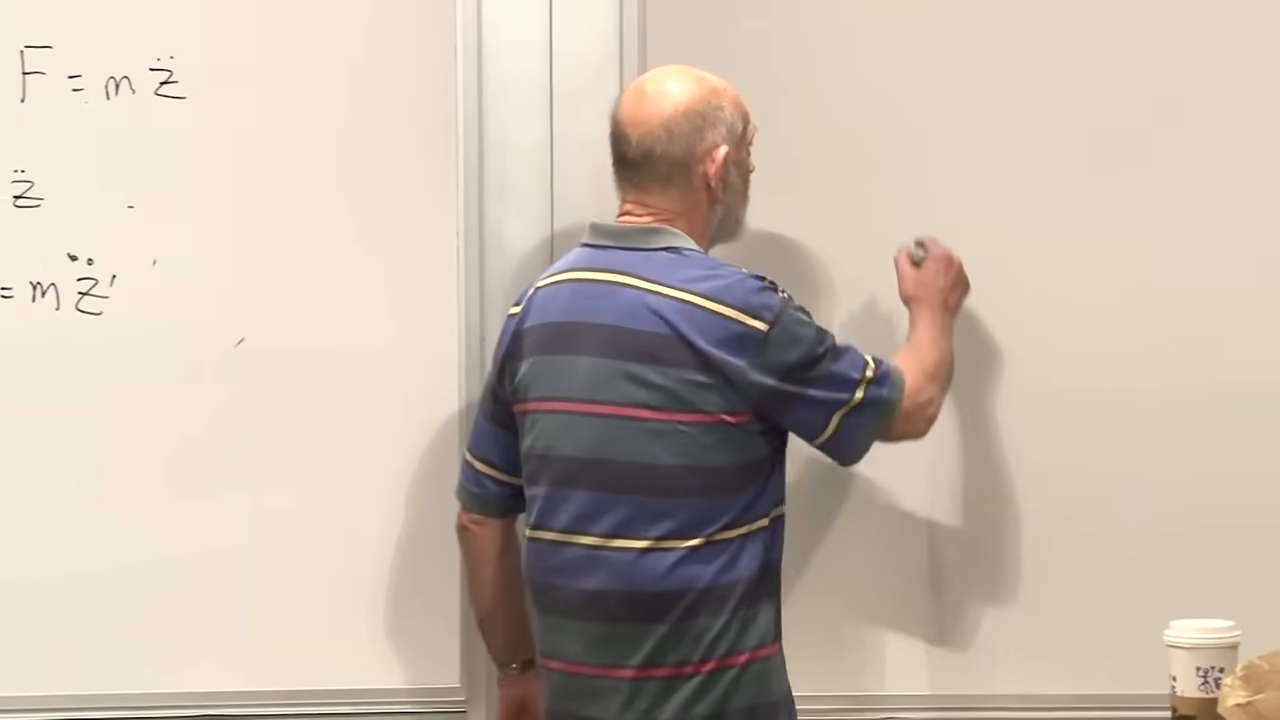
\includegraphics[width=\linewidth]{lecture_01_figure_02.png}
\caption{兩個等速運動座標系中的牛頓方程。}
\par\smallskip
\textit{課堂畫面：00:11:50。}
\end{figure}

現在讓電梯以固定的\(g\)向上加速：
\begin{equation}
 L(t)=\frac12gt^2,\qquad
 \dot L=gt,\qquad
 \ddot L=g.
\end{equation}
座標變換變為
\begin{equation}
 z'=z-\frac12gt^2,
\qquad
 \ddot z'=\ddot z-g.
\label{eq:accelerated-map}
\end{equation}
代入牛頓定律可得
\begin{equation}
 F=m(\ddot z'+g),
\qquad
 m\ddot z'=F-mg.
\label{eq:fictitious-gravity}
\end{equation}
這個推導也提供了一個實用的符號檢查：\(+mg\)先出現在加速度那一側，移到力那一側後才變成\(-mg\)。在地板向上加速的參考系中，最後得到的方向是向下。

\begin{figure}[H]
\centering
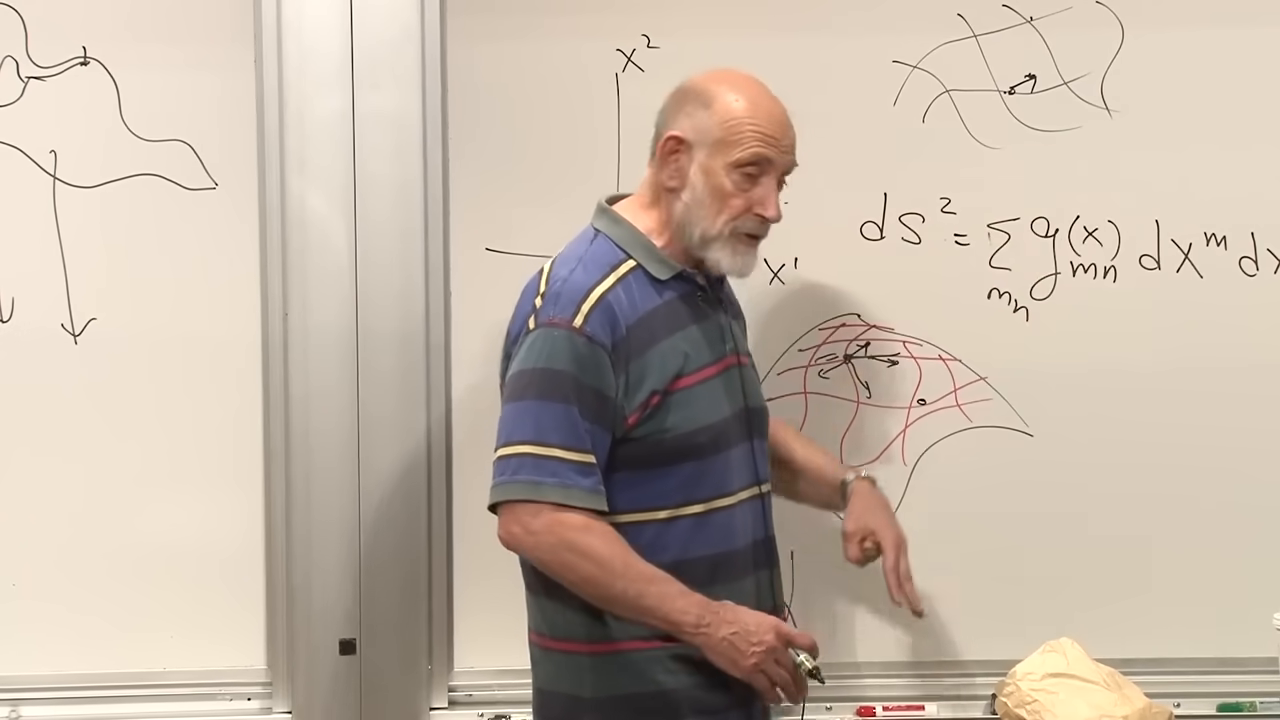
\includegraphics[width=\linewidth]{lecture_01_figure_03.png}
\caption{加速座標變換及其導出的假想力\(-mg\)。}
\par\smallskip
\textit{課堂畫面：00:15:35。}
\end{figure}

新增項之所以看起來像重力，有一個明確的原因：它與質量成正比。慣性反應也與質量成正比，因此質量會從運動方程中消去。自由落體的軌跡不因物體的質量而異。例如，在試驗物體近似下，地球的軌道由它在太陽重力場中的位置與速度決定，而非由地球自身的質量決定。

在愛因斯坦之前，這種相似之處或許只會被視為奇特的巧合。愛因斯坦卻將它提升為一項原理：任何局部力學實驗都無法區分均勻重力場與適當加速的參考系。

\section{直線、彎曲座標與光}

將\(t\)軸畫成垂直方向，\(z\)軸畫成水平方向。對於
\(z'=z-vt\)，\(z'\)固定不變的線是彼此平行的直線。
直線世界線仍是直線，因為座標變換是線性的。

\begin{figure}[H]
\centering
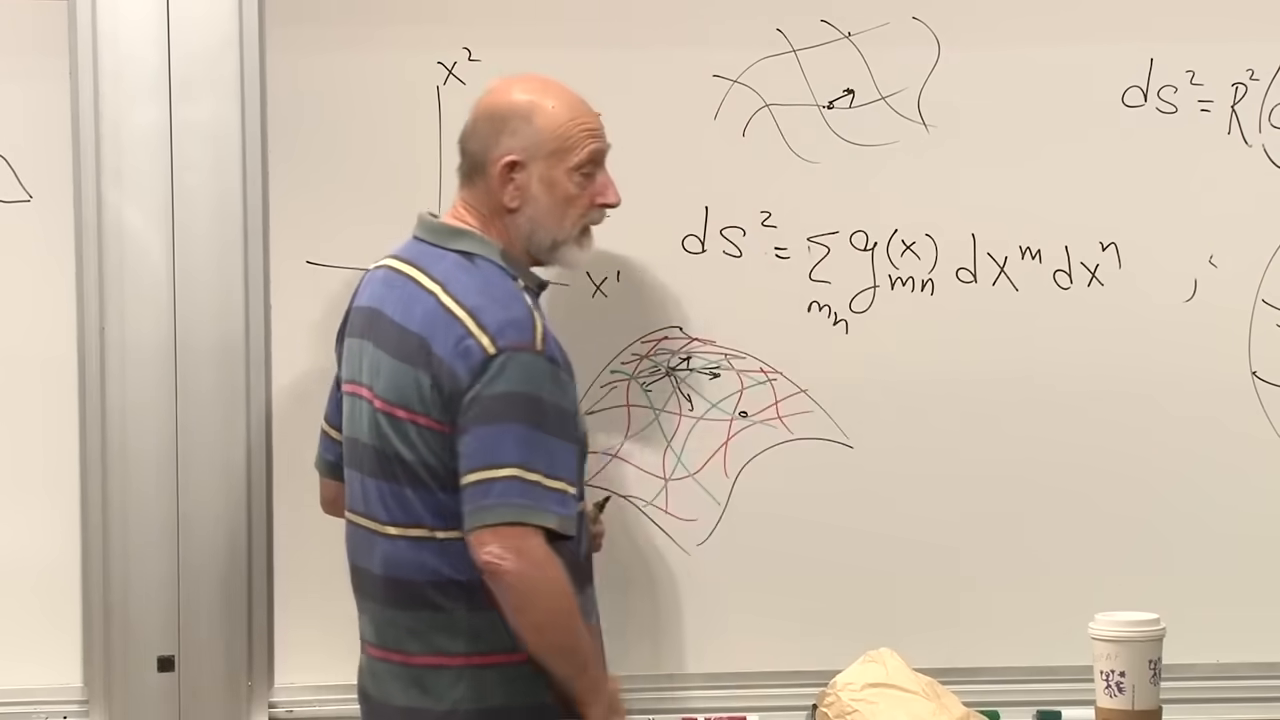
\includegraphics[width=\linewidth]{lecture_01_figure_04.png}
\caption{等速運動座標系的線性時空網格。}
\par\smallskip
\textit{課堂畫面：00:19:45。}
\end{figure}

對加速座標變換而言，\(z'\)固定不變的線滿足
\begin{equation}
 z=z'+\frac12gt^2.
\end{equation}
這是一條側躺的拋物線。把運動向過去延伸，電梯會先下降並減速，接著轉向，再向上加速。每一條相鄰的\(z'\)固定線，都是同一條拋物線向水平方向平移而成。

\begin{figure}[H]
\centering
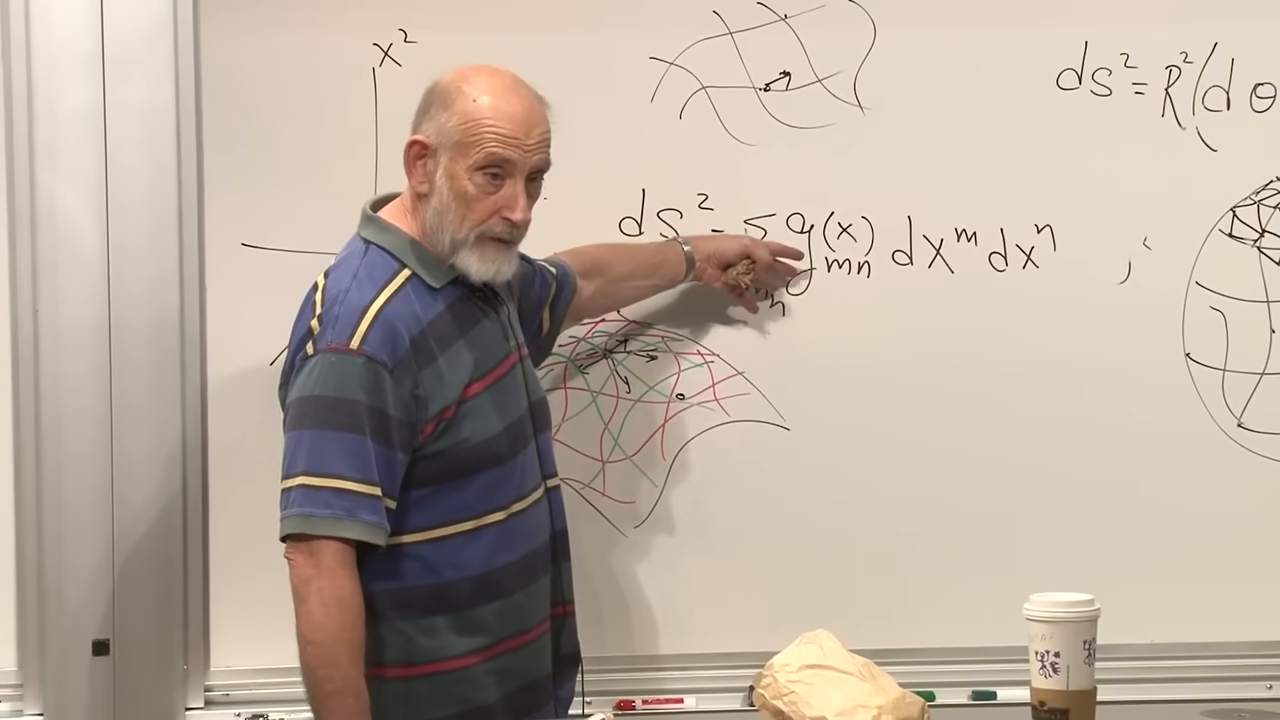
\includegraphics[width=\linewidth]{lecture_01_figure_05.png}
\caption{等加速度座標系中的\(z'\)固定曲線。}
\par\smallskip
\textit{課堂畫面：00:22:25。}
\end{figure}

這是第一個幾何線索。狹義相對論使用線性的洛倫茲變換，而這種變換會將時空中的直線映成直線。要描述加速度，進而模擬重力，就需要對時空座標施行曲線變換。

愛因斯坦運用這個看似不起眼的論點，回答了一個極為重要的問題：重力會影響光嗎？在\(t=0\)，令電梯參考系與地面參考系瞬間相對靜止，並讓一束水平光線穿過電梯。在未加速的參考系中，
\begin{equation}
 x=ct,\qquad z=0.
\end{equation}
利用\(z=z'+\tfrac12gt^2\)，同一束光在電梯座標中滿足
\begin{equation}
 z'=-\frac12gt^2
    =-\frac{g}{2c^2}x^2.
\label{eq:accelerated-light}
\end{equation}
光線在慣性系中是直的，在加速系中則是彎的。如果加速度與重力在局部等效，重力場就必定會使光線彎曲。這個論證在寫出重力場方程之前，就已經確立了這項效應。

\begin{figure}[H]
\centering
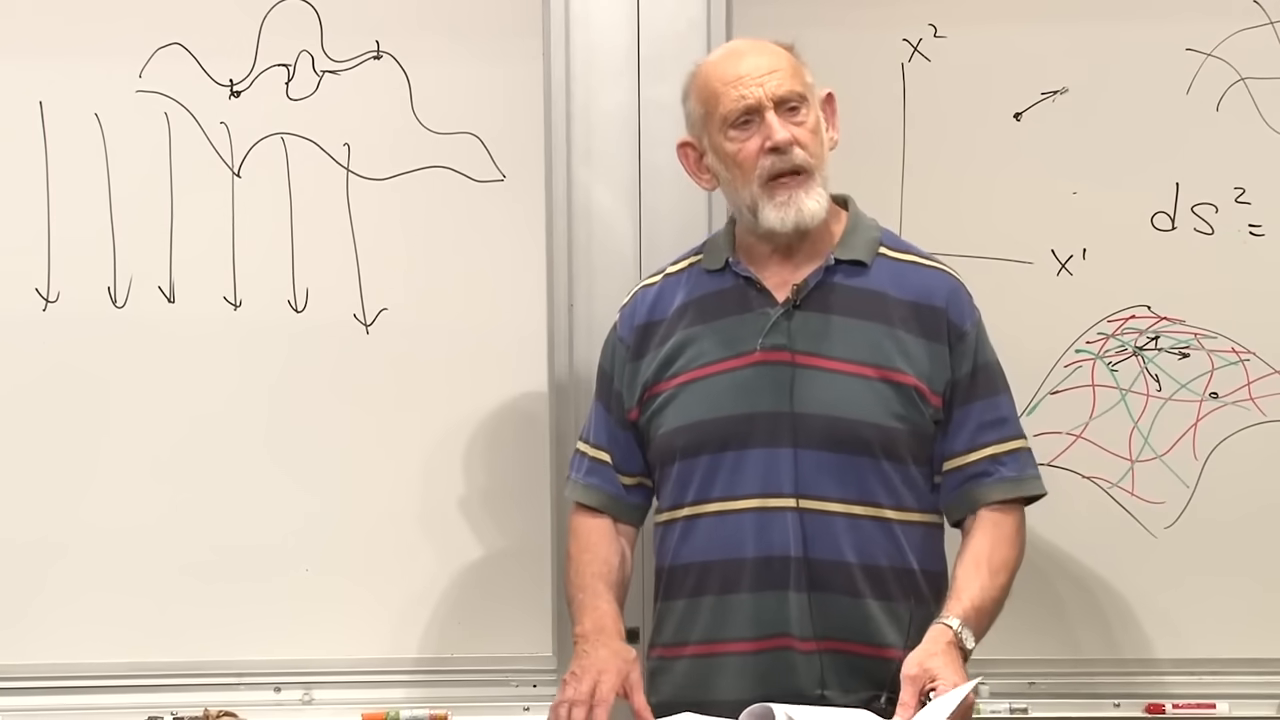
\includegraphics[width=\linewidth]{lecture_01_figure_06.png}
\caption{水平光線及其在加速參考系中的彎曲軌跡。}
\par\smallskip
\textit{課堂畫面：00:28:10。}
\end{figure}

\section{無法透過座標變換消除的效應}

加速參考系可以產生表觀的均勻重力場，但這不表示所有重力場都是座標造成的假象。恆星的重力場沿徑向指向內側。在恆星附近某一點周圍的小型自由落體實驗室，可以消除該處的局部加速度，但同一個座標變換無法消除恆星四周各處的重力場。

\begin{figure}[H]
\centering
\includegraphics[width=\linewidth]{lecture_01_figure_07.png}
\caption{徑向重力場與用來顯示潮汐加速度的延展自由落體物體。}
\par\smallskip
\textit{課堂畫面：00:32:50。}
\end{figure}

問題在於潮汐力。想像有個身高兩千英里的人頭朝上自由下落。他的腳比頭更靠近重力源，因此加速度更大，身體便會被拉長。若他側身下落，兩側朝內的方向分量會彼此相向，因此身體會被擠壓。用牛頓力學的說法，相隔\(\xi^j\)的相鄰點會產生相對加速度
\begin{equation}
 \delta a^i \simeq \partial_j g^i\,\xi^j.
\label{eq:newtonian-tide}
\end{equation}
座標加速度可以消除，但延展的自由落體物體各部分之間的相對加速度無法消除。

\begin{classroomqa}
\audiencequestion{如果在頭部和腳部分別使用不同的火箭引擎，能否模擬拉伸，進而模擬潮汐場？}
\lecturerresponse{引擎當然能對物體施力，但那是真實的非重力作用力，而且對物體各部分的作用不同。單靠座標變換，無法在相鄰的自由落體粒子之間產生不變的相對加速度。這項判準針對的是不受外力的自由落體，而不是由不同火箭引擎推動的物體。
\lecturetimestamp{00:36:51}}
\end{classroomqa}

不過，彎曲座標仍能讓假想場看起來相當複雜。某個參考系可以在垂直方向加速，同時在水平方向振盪，形成包含兩個分量且隨時間變化的表觀場。即使是一般的極座標，也能說明這點。一個沿笛卡兒座標中的直線運動的自由粒子，其\(r(t)\)先減小，到達最小半徑後，再逐漸\(r(t)\)增大。若只知道\(r(t)\)和\(\theta(t)\)，觀察者可能會推斷有一個向外的斥力。在這類座標的旋轉版本中，還會出現離心項與科里奧利項。它們與質量成正比，因此看起來像重力，但不會在自由落體物體上留下不變的潮汐應變。

\begin{classroomqa}
\audiencequestion{如果用角座標或極座標來描述運動，會發生什麼事？}
\lecturerresponse{非線性的座標描述會讓直線自由軌跡看起來像是受到\(r=0\)排斥。這種有效的離心力是座標力。回到慣性笛卡兒座標系便會消除此力，顯示並沒有潮汐形變。
\lecturetimestamp{00:37:56}}
\end{classroomqa}

\begin{figure}[H]
\centering
\includegraphics[width=\linewidth]{lecture_01_figure_08.png}
\caption{直線軌跡的極座標描述，板書標出了\(r(t)\)和\(\theta(t)\)。}
\par\smallskip
\textit{課堂畫面：00:40:20。}
\end{figure}

\begin{classroomqa}
\audiencequestion{多個重力源能否彼此抵消，使潮汐力完全消失？}
\lecturerresponse{各力可以在選定的一點抵消，但場值抵消通常不會使其空間導數也抵消。在任何一個重力源附近，相鄰的軌跡仍會因而獲得不同的加速度。若要真正沒有曲率，整個區域內的潮汐判準都必須為零，而不能只是在某一點的合力為零。\lecturetimestamp{00:42:16}}
\end{classroomqa}

\begin{classroomqa}
\audiencequestion{如何以實際操作測量潮汐力？}
\lecturerresponse{讓一個有延展性的物體（例如晶體）自由落體，觀察是否出現使它在一個方向拉長、在另一個方向壓縮的應力與應變。這些形變可以測量，也不會因為更改座標名稱而消失。\lecturetimestamp{00:44:38}}
\end{classroomqa}

\begin{classroomqa}
\audiencequestion{一個身高兩千英里的人坐在旋轉木馬上，會感受到徑向潮汐效應嗎？}
\lecturerresponse{被固定在旋轉木馬上的人會感受到支撐力，也可能真的頭痛。但測試物體必須處於自由落體。它的軌跡在旋轉座標中看來很複雜，在慣性系中卻仍是一條不受應力的直線軌跡，因此不變的潮汐力為零。
\lecturetimestamp{00:45:07}}
\end{classroomqa}

\begin{classroomqa}
\audiencequestion{能否傾斜下落物體，讓拉伸與擠壓互相抵消？}
\lecturerresponse{沒有任何單一取向能消除全部形變。徑向重力場沿一個主方向拉伸物體，並沿橫向方向壓縮。在所有方向上都有有限延展的物體會經歷完整的形變模式。\lecturetimestamp{00:47:10}}
\end{classroomqa}

\begin{figure}[H]
\centering
\includegraphics[width=\linewidth]{lecture_01_figure_09.png}
\caption{延展的自由落體物體同時呈現徑向拉伸與橫向壓縮。}
\par\smallskip
\textit{課堂畫面：00:47:55。}
\end{figure}

\begin{classroomqa}
\audiencequestion{潮汐力是否表示等效原理失效？}
\lecturerresponse{潮汐力說明了表述等效原理時必須多麼謹慎。若系統小到重力場在其範圍內的變化可以忽略，就能以自由落體參考系在所需精度內消除重力。較大系統內殘留的變化就是潮汐場。\lecturetimestamp{00:48:08}}
\end{classroomqa}

\section{從閔可夫斯基幾何到局部度規}

現在我們暫時離開重力，稍作停頓。閔可夫斯基早已指出，時空具有不變的局部幾何。在一維空間中，取\(c=1\)，
\begin{equation}
 d\tau^2=dt^2-dx^2.
\label{eq:minkowski-proper-time}
\end{equation}
也可以改為定義\(ds^2=dx^2-dt^2=-d\tau^2\)。兩者的差異只是號差慣例不同，並非物理有所不同。

\begin{classroomqa}
\audiencequestion{如果不把光速設為 1，它應該出現在哪裡？}
\lecturerresponse{若\(t\)以時間為單位測量，而\(x\)以長度為單位測量，一種方便的寫法是
\(d\tau^2=dt^2-dx^2/c^2\)。等價地，乘上\(c^2\)並使用
\(c^2d\tau^2=c^2dt^2-dx^2\)。選用\(ct\)或\(x/c\)作為座標，就能吸收這個換算因子。\lecturetimestamp{00:51:02}}
\end{classroomqa}

\begin{figure}[H]
\centering
\includegraphics[width=\linewidth]{lecture_01_figure_10.png}
\caption{固有時間間隔為幾何提供了橋樑，使狹義相對論得以連接到廣義相對論。}
\par\smallskip
\textit{課堂畫面：00:51:10。}
\end{figure}

愛因斯坦發現，判斷重力場是否可被消除的問題，與高斯研究曲面、黎曼研究任意維度時所探討的問題相似：給定局部距離定律，要如何判斷幾何是否真正彎曲？

在歐幾里得笛卡兒座標中，畢氏定理給出
\begin{equation}
 ds^2=(dx^1)^2+(dx^2)^2+\cdots
     =\delta_{mn}\,dx^m dx^n.
\label{eq:euclidean-line-element}
\end{equation}
指標的取值範圍就是空間的維度。無論座標有二個、三個或二十六個，這套記號都不必改變。

\begin{figure}[H]
\centering
\includegraphics[width=\linewidth]{lecture_01_figure_11.png}
\caption{歐幾里得線元素：座標微分的平方和。}
\par\smallskip
\textit{課堂畫面：00:55:00。}
\end{figure}

在任意曲面上採用任意座標\(x^m\)。相鄰點之間的距離由二次型給出：
\begin{equation}
 ds^2=g_{mn}(x)\,dx^m dx^n.
\label{eq:general-line-element}
\end{equation}
函數\(g_{mn}(x)\)是度規張量的分量。同一公式也適用於使用曲線座標描述的平坦曲面；度規分量不是常數，本身並不能證明存在內在曲率。

\begin{figure}[H]
\centering
\includegraphics[width=\linewidth]{lecture_01_figure_12.png}
\caption{一般度規二次型與彎曲座標網格。}
\par\smallskip
\textit{課堂畫面：00:58:20。}
\end{figure}

對於半徑為\(R\)的球面，若\(\theta\)是從某一極點量起的角度，則
\begin{equation}
 ds^2=R^2\left(d\theta^2+\sin^2\theta\,d\phi^2\right).
\label{eq:sphere-polar}
\end{equation}
相同的經度增量在赤道附近跨越的距離較長，在極點附近跨越的距離較短；係數正是記錄這種位置依賴性。

\begin{classroomqa}
\audiencequestion{一般所說的緯度是從赤道量起的，那麼係數應該是餘弦，而不是正弦嗎？}
\lecturerresponse{是的。若\(\lambda\)表示從赤道量起的緯度，那麼
\(ds^2=R^2(d\lambda^2+\cos^2\lambda\,d\phi^2)\)。
方程\eqref{eq:sphere-polar}使用的是從北極量起的極角
\(\theta=\pi/2-\lambda\)。
\lecturetimestamp{01:01:03}}
\end{classroomqa}

\begin{figure}[H]
\centering
\includegraphics[width=\linewidth]{lecture_01_figure_13.png}
\caption{球面度規，以及決定位置相關係數的緯度--經度幾何。}
\par\smallskip
\textit{課堂畫面：01:00:30。}
\end{figure}

更一般的座標可以引入\(d\theta\,d\phi\)交叉項，但局部距離對微分仍是二次形式。三次項或一次項不屬於黎曼線元素。

\section{局部距離與內在曲率}

\begin{classroomqa}
\audiencequestion{度規公式也能直接給出相距甚遠的兩點之間的距離嗎？}
\lecturerresponse{不能直接代入求得。它給出的是相鄰點之間的距離。宏觀距離需要指定路徑，並對\(ds\)積分；如果所說的距離是最短路徑長度，就必須根據幾何求出這條路徑。同一對端點甚至可能由多條局部最短路徑連接。\lecturetimestamp{01:02:30}}
\end{classroomqa}

想像在一個崎嶇的曲面上，於相距甚遠的兩點打入樁子，再把一條繃緊的繩子繫在兩樁之間。繩子可能繞過山丘的一側，也可能繞過另一側；移動山丘會改變使路徑長度最小的路線。全域距離取決於兩點之間的幾何。局部距離則較簡單：度規在每一點提供一把小尺，幾何便由這些無窮小的尺組合而成。

\begin{figure}[H]
\centering
\includegraphics[width=\linewidth]{lecture_01_figure_14.png}
\caption{全域距離問題：繃緊的路徑必須沿著曲面穿越兩個端點之間的區域。}
\par\smallskip
\textit{課堂畫面：01:04:00。}
\end{figure}

如果局部的小片能不經拉伸或撕裂就鋪在平面上，內在幾何便是平坦的。具有球面三角網格邊長的小片，無法在保留所有邊長的情況下全部鋪平。因此，度規提出了一個明確問題：給定\(g_{mn}(x)\)，能否判定其無窮小部分是否能像平坦空間一樣拼合？

\begin{figure}[H]
\centering
\includegraphics[width=\linewidth]{lecture_01_figure_15.png}
\caption{度規與局部座標區塊：構成幾何的無窮小部分。}
\par\smallskip
\textit{課堂畫面：01:05:20。}
\end{figure}

\begin{classroomqa}
\audiencequestion{能否透過測量圓周長與直徑的比值來判斷曲率？}
\lecturerresponse{可以，這是很有用的二維檢驗。在彎曲曲面上，這個比值可能不同於\(\pi\)。不過，對無窮小圓而言，偏差要到較高階才會出現；而且與曲率張量相比，這種方法較難推廣。
\lecturetimestamp{01:07:26}}
\end{classroomqa}

如果存在一個座標系，使得整個區域內處處滿足
\begin{equation}
 g_{mn}=\delta_{mn},
\qquad
 ds^2=\delta_{mn}\,dx^m dx^n
\label{eq:flat-metric}
\end{equation}
那麼該區域就是平坦的。因此，複雜的\(g_{mn}(x)\)可能描述彎曲空間，也可能只是在平坦空間中使用彎曲座標。關鍵在於能否藉由座標變換消除所有這些複雜性。

\begin{figure}[H]
\centering
\includegraphics[width=\linewidth]{lecture_01_figure_16.png}
\caption{在局部座標區塊上陳述度規問題：能否將它的曲線座標形式變換為平坦形式？}
\par\smallskip
\textit{課堂畫面：01:07:15。}
\end{figure}

\begin{classroomqa}
\audiencequestion{球面線元素是否假設每個小區間都是平坦的，儘管球面本身並不平坦？}
\lecturerresponse{在最低階近似下，每個光滑曲面在一點附近都可以用該點的切平面近似。曲率表現在相鄰的切平面近似無法彼此拼合，或表現在有限區域內的高階變化。因此，局部的歐幾里得行為與全域曲率並不矛盾。\lecturetimestamp{01:10:01}}
\end{classroomqa}

\begin{classroomqa}
\audiencequestion{度規必須連續嗎？摺痕或裂隙處會如何？}
\lecturerresponse{這裡的討論假設座標映射與度規足夠光滑，能進行所需的微分。紙張摺疊時若不拉伸，摺痕兩側的內在距離仍相同；引人注目的外觀變化屬於外在幾何。真正奇異或不光滑的幾何需要另外處理，超出這裡採用的光滑架構。\lecturetimestamp{01:11:25}}
\end{classroomqa}

這就是內在幾何與外在幾何的區別。在三維空間中彎折一頁紙會改變它的嵌入方式，卻不會改變沿紙面測得的距離。即使某種生物只能待在紙面上，無法觀察嵌入空間，它仍能測量紙面的內在幾何。

\begin{figure}[H]
\centering
\includegraphics[width=\linewidth]{lecture_01_figure_17.png}
\caption{用摺疊紙張說明內在距離與外在外觀的差異。}
\par\smallskip
\textit{課堂畫面：01:13:00。}
\end{figure}

\begin{classroomqa}
\audiencequestion{為什麼不直接將度規對角化？}
\lecturerresponse{在任一點上，適當選擇座標就能將度規對角化，並將其規範化為局部平坦形式。難處在於，能否使用同一套座標在整個區域內都做到這一點。只檢查單一點，無法判定曲率。
\lecturetimestamp{01:13:48}}
\end{classroomqa}

\begin{figure}[H]
\centering
\includegraphics[width=\linewidth]{lecture_01_figure_18.png}
\caption{一般局部二次型下方寫出的平坦笛卡兒度規\(\delta_{mn}\)。}
\par\smallskip
\textit{課堂畫面：01:16:00。}
\end{figure}

此時，重力與幾何的類比已是精確的，而不只是暗示。座標力可以消除，正如平坦空間中的曲線座標描述可以消除。在廣義相對論中，曲率用來描述潮汐加速度。以後續會使用的記號表示，相鄰的自由落體世界線滿足測地線偏離方程
\begin{equation}
 \frac{D^2\xi^\mu}{D\tau^2}
 =-R^\mu{}_{\nu\rho\sigma}
   u^\nu\xi^\rho u^\sigma.
\label{eq:geodesic-deviation-preview}
\end{equation}
曲率為零表示不存在不變的潮汐場；曲率非零則表示無法透過任何座標選擇消除整個區域內的重力。

\section{兩個座標系與一個向量}

要判斷度規能否變換為\(\delta_{mn}\)，我們必須先了解幾何物件如何變換。令\(x^m\)與\(y^m\)為同一區域上的兩套光滑座標系：
\begin{equation}
 x^m=x^m(y),\qquad y^m=y^m(x).
\label{eq:mutual-coordinate-maps}
\end{equation}
符號\(x\)與\(y\)代表完整的座標系，而非兩個特定的空間方向。

\begin{figure}[H]
\centering
\includegraphics[width=\linewidth]{lecture_01_figure_19.png}
\caption{彼此相關的座標映射\(x^m(y)\)與\(y^m(x)\)。}
\par\smallskip
\textit{課堂畫面：01:20:35。}
\end{figure}

對相鄰點使用鏈鎖律可得
\begin{equation}
 dy^m=\frac{\partial y^m}{\partial x^p}\,dx^p.
\label{eq:differential-transform}
\end{equation}
重複出現的指標\(p\)代表求和。位移本身是同一個幾何向量；\(dx^p\)與\(dy^m\)則是它在兩套座標系中的分量。

\begin{figure}[H]
\centering
\includegraphics[width=\linewidth]{lecture_01_figure_20.png}
\caption{由鏈鎖律得到的微分座標變換。}
\par\smallskip
\textit{課堂畫面：01:22:30。}
\end{figure}

\begin{classroomqa}
\audiencequestion{在曲線座標網格上，座標線代表什麼？}
\lecturerresponse{在二維情況下，固定一個座標而讓另一個座標變動，就會得到一條線。在更高維度中，相應的定座標集合是超曲面。這些集合的局部交會，定義了解析向量分量時所用的座標方向。\lecturetimestamp{01:25:20}}
\end{classroomqa}

逆變向量依照與座標位移相同的變換律定義：
\begin{equation}
 (V')^m(y)
 =\frac{\partial y^m}{\partial x^p}\,V^p(x).
\label{eq:contravariant-vector}
\end{equation}
沿曲面的速度就是一個例子。座標改變時，向量本身不變，改變的是它的分量。

\begin{figure}[H]
\centering
\includegraphics[width=\linewidth]{lecture_01_figure_21.png}
\caption{以方框標示的逆變向量變換律。}
\par\smallskip
\textit{課堂畫面：01:29:30。}
\end{figure}

愛因斯坦求和約定規定：若同一指標一次出現在上標、一次出現在下標，就省略求和符號。這項約定讓公式較容易排版；更重要的是，它使縮併的模式一目了然。

\begin{classroomqa}
\audiencequestion{對允許使用的座標系，是否作了什麼特殊假設？}
\lecturerresponse{只假設兩套座標系之間有函數關係，而且在所討論的區域內足夠光滑，使得式中所列的導數與反函數映射存在。並未假設它們是線性的或正交的。\lecturetimestamp{01:28:12}}
\end{classroomqa}

\section{協向量與鏈鎖律}

令\(S(x)\)為一個純量：它在每一點都有明確的值，不受座標標記影響。溫度和純量場都是例子。它的梯度分量為
\begin{equation}
 W_p=\frac{\partial S}{\partial x^p}.
\label{eq:gradient-covector}
\end{equation}

\begin{figure}[H]
\centering
\includegraphics[width=\linewidth]{lecture_01_figure_22.png}
\caption{在逆變變換律旁引入純量梯度。}
\par\smallskip
\textit{課堂畫面：01:31:40。}
\end{figure}

在\(y\)座標中套用鏈鎖律，
\begin{equation}
 W'_m
 =\frac{\partial S}{\partial y^m}
 =\frac{\partial x^p}{\partial y^m}
  \frac{\partial S}{\partial x^p}
 =\frac{\partial x^p}{\partial y^m}\,W_p.
\label{eq:covariant-vector}
\end{equation}
這就是協變向量（或稱協向量）的變換律。這裡的雅可比矩陣是\eqref{eq:contravariant-vector}中雅可比矩陣的反矩陣，因此，下標與上標代表不同的變換行為。

\begin{figure}[H]
\centering
\includegraphics[width=\linewidth]{lecture_01_figure_23.png}
\caption{並列顯示的逆變與協變變換律。}
\par\smallskip
\textit{課堂畫面：01:34:40。}
\end{figure}

\begin{classroomqa}
\audiencequestion{協變向量與逆變向量之間有什麼關係？}
\lecturerresponse{在這個階段，它們被定義為不同種類的物件：位移和速度依一種方式變換，梯度則依相反的方式變換。稍後，度規會提供一種一對一的對應，用來升降指標。在引入度規之前，不應預先假定兩者有這種關係。\lecturetimestamp{01:37:43}}
\end{classroomqa}

\begin{classroomqa}
\audiencequestion{此前降低指標時，時間分量的符號是否曾經改變？}
\lecturerresponse{那個符號來自洛倫茲度規。目前的推導先在普通的歐幾里得幾何中進行。升高或降低指標一律使用相應的度規；只有度規具有洛倫茲號差時，時間分量才會出現負號。
\lecturetimestamp{01:38:29}}
\end{classroomqa}

\begin{classroomqa}
\audiencequestion{現在是否應該把這兩條變換律視為同一個向量的兩種分量描述？}
\lecturerresponse{還不能。有了度規之後，才能將逆變向量 \(V^m\) 轉換為協變向量 \(V_m=g_{mn}V^n\)。在建立這種對應之前，上指標與下指標的物件在邏輯上是不同的。\lecturetimestamp{01:39:00}}
\end{classroomqa}

這些公式與維度無關。指標的範圍會隨維度改變，但變換律不變。

\section{多重指標張量}

取兩個逆變向量 \(V^m\) 和 \(U^n\)。它們的乘積
\begin{equation}
 T^{mn}=V^mU^n
\label{eq:rank-two-product}
\end{equation}
是一個二階逆變張量。在三維空間中，它有九個分量；在四維空間中，則有十六個分量。除非另有對稱性條件，否則指標的次序很重要：\(T^{mn}\)不必等於 \(T^{nm}\)。

\begin{figure}[H]
\centering
\includegraphics[width=\linewidth]{lecture_01_figure_24.png}
\caption{由兩個逆變向量相乘構成的二階張量。}
\par\smallskip
\textit{課堂畫面：01:43:40。}
\end{figure}

每個上指標都會帶來一個正向雅可比因子：
\begin{equation}
 (T')^{mn}
 =\frac{\partial y^m}{\partial x^p}
  \frac{\partial y^n}{\partial x^q}
  T^{pq}.
\label{eq:rank-two-contravariant}
\end{equation}
乘積的構造說明了這條規則，但張量的定義在於其變換律。三階逆變張量會帶有三個這樣的雅可比因子。

\begin{figure}[H]
\centering
\includegraphics[width=\linewidth]{lecture_01_figure_25.png}
\caption{變換 \(T^{mn}\) 時出現的兩個雅可比因子。}
\par\smallskip
\textit{課堂畫面：01:44:20。}
\end{figure}

同樣地，每個下指標都會帶來一個逆雅可比因子：
\begin{equation}
 T'_{mn}
 =\frac{\partial x^p}{\partial y^m}
  \frac{\partial x^q}{\partial y^n}
  T_{pq}.
\label{eq:rank-two-covariant}
\end{equation}
混合張量則各帶有一個正向與逆雅可比因子。

\begin{figure}[H]
\centering
\includegraphics[width=\linewidth]{lecture_01_figure_26.png}
\caption{具有兩個協變指標的張量之完整變換律。}
\par\smallskip
\textit{課堂畫面：01:47:30。}
\end{figure}

同樣的變換機制現在也適用於度規。由於線元是純量，它在兩個座標系中必須具有相同的值：
\begin{align}
 ds^2
 &=g_{mn}(x)\,dx^m dx^n,\\
 dx^m
 &=\frac{\partial x^m}{\partial y^p}\,dy^p.
\end{align}
代入後，就補上了黑板上未完成的那一行：
\begin{equation}
 g'_{pq}(y)
 =\frac{\partial x^m}{\partial y^p}
  \frac{\partial x^n}{\partial y^q}
  g_{mn}(x(y)).
\label{eq:l1-metric-transformation}
\end{equation}
因此，\(g_{mn}\)是二階協變張量。

\begin{figure}[H]
\centering
\includegraphics[width=\linewidth]{lecture_01_figure_27.png}
\caption{講座結尾從線元不變性出發推導的度規變換。}
\par\smallskip
\textit{課堂畫面：01:48:40。}
\end{figure}

一開始提出的物理問題，現在轉化成了數學問題。給定 \(g_{mn}(x)\)，是否存在一種座標變換，使得在整個區域內 \(g'_{mn}=\delta_{mn}\)？若存在，表面上的複雜性就只是座標造成的複雜性。若不存在，阻礙便是曲率；在時空中，這種阻礙就是引力的不變內容。